%implementing document formatting:
%page setup (page size, text size, page layout, chapters start on a new page).
%memoir is a form of book class that supports any kind of document.
\documentclass[fleqn,a4paper,12pt,twoside,openany]{memoir}


%%%%%%%%%%%%%%%%% Prøver mig lidt frem

%%%%%%%%%%%%%%%%%%%%%%%%%%%%%%%%%%%%%%%%%%%%%%%%%5


%setting the header and footer in that order:
\setheadfoot{28pt}{28pt} %if any problems are encountered, try changing the latter 28pt with 1cm.

%general package syntax: \usepackage[options]{package}

%setting language:
%\usepackage[danish]{babel}  -- Gamle
\RequirePackage[danish]{babel}

%this package makes it possible to treat any element as a float,
%figures and tables are by default treated as floats.
%read http://en.wikibooks.org/wiki/LaTeX/Floats,_Figures_and_Captions to specify your float.
\usepackage{float}
\usepackage{wrapfig}
\usepackage{placeins}

\usepackage{multirow}

%this package makes it possible to make theorems and examples:
\usepackage{amsthm}
%setting the style of examples (parameters: plain, definition, remark):
%(definition is usually used for examples)
\theoremstyle{definition}
%the frist parameter is the syntax used in the document, the second is that which is printed in LaTex.
\newtheorem{example}{Eksempel}

%making it possible to use æ, ø and å:
\usepackage[utf8]{inputenc}
%helps with word division when using æ, ø and å, and makes it ps-font rather than bmp:
\usepackage[T1]{fontenc}

%package for implementation of graphic files:
\usepackage{graphicx}

%package for captions
\usepackage[nooneline]{caption}

%%package for implementation of math:
\usepackage{amsmath , amsfonts , amssymb, float}

%allowing use of color:
\usepackage{color}
%allowing use of more colors also in tables (see: http://en.wikibooks.org/wiki/LaTeX/Colors):
\usepackage[usenames,dvipsnames,svgnames,table]{xcolor}

%hyperlinks in the tabel of contents - comment this out before the report is printed.
\usepackage{hyperref}
\hypersetup{
	bookmarks = true,  % Show 'bookmark'-frame in pdf.
	colorlinks = true, % True = colored links, False = framed links.
	citecolor = black,  % Link color for references.
	linkcolor = black,  % Link color in table of contents.
	urlcolor = black,   % Link color for extern URLs.
}

%makes it possible to refer to the name of a chapter rather than just the number.
\usepackage{nameref}

%package for writing program code in latex
\usepackage{listings}

\lstset{ 
language=C,               	 	% choose the language of the code
basicstyle=\footnotesize,       % the size of the fonts that are used for the code
numbers=left,                   % where to put the line-numbers
numberstyle=\footnotesize,      % the size of the fonts that are used for the line-numbers
stepnumber=1,                   % the step between two line-numbers. If it is 1 each line will be numbered
numbersep=5pt,                  % how far the line-numbers are from the code
backgroundcolor=\color{white},  % choose the background color. You must add \usepackage{color}
showspaces=false,               % show spaces adding particular underscores
showstringspaces=false,         % underline spaces within strings
showtabs=false,                 % show tabs within strings adding particular underscores
frame=single,           		% adds a frame around the code
tabsize=2,          			% sets default tabsize to 2 spaces
captionpos=b,           		% sets the caption-position to bottom
breaklines=true,       			% sets automatic line breaking
breakatwhitespace=false,    	% sets if automatic breaks should only happen at whitespace
escapeinside={\%*}{*)}          % if you want to add a comment within your code
}

%setting references (using numbers) and supporting i.a. Chicargo-style:
\usepackage{etex}
\usepackage{etoolbox}
\usepackage{keyval}
\usepackage{ifthen}
\usepackage{url}
\usepackage{csquotes}
\usepackage[numbers]{natbib}
\bibliographystyle{plain}
\newcommand{\btx}{Bib\TeX}
%\usepackage[backend=biber,url=true,doi=true,style=numeric, sorting=none]{biblatex}
%\addbibresource{VoresKilder.bib}

%this package makes it possible include pdf pages in fx appendix;
%using  following syntax: \includepdf[pages={1}]{myfile.pdf}
\usepackage{pdfpages}

%%%MARGINER%%%
\setlrmarginsandblock{3.5cm}{2.5cm}{*}	% \setlrmarginsandblock{inner margin}{outer margin}{ratio}
\setulmarginsandblock{2.5cm}{3.0cm}{*}	% \setulmarginsandblock{top}{bottom}{ratio}
\checkandfixthelayout 			            % fixes stuff..

%Enables the use FiXme refferences. Syntax: \fixme{...}
%With "final" in stead of "draft" an error will ocure for every FiXme
%under compilation.
\usepackage[footnote,draft,english,silent,nomargin]{fixme}

%%%CHAPTERLAYOUT%%%
%setting the color of the chapter number
\definecolor{numbercolor}{gray}{0.7}
%Downloaded chapter-setup:
\newif\ifchapternonum
\makechapterstyle{jenor}{
  \renewcommand\printchaptername{}
  \renewcommand\printchapternum{}
  \renewcommand\printchapternonum{\chapternonumtrue}
  \renewcommand\chaptitlefont{\fontfamily{pbk}\fontseries{db}\fontshape{n}\fontsize{25}{35}\selectfont\raggedleft}
  \renewcommand\chapnumfont{\fontfamily{pbk}\fontseries{m}\fontshape{n}\fontsize{1in}{0in}\selectfont\color{numbercolor}}
  \renewcommand\printchaptertitle[1]{%
    \noindent
    \ifchapternonum
    \begin{tabularx}{\textwidth}{X}
    {\let\\\newline\chaptitlefont ##1\par} 
    \end{tabularx}
    \par\vskip-2.5mm\hrule
    \else
    \begin{tabularx}{\textwidth}{Xl}
    {\parbox[b]{\linewidth}{\chaptitlefont ##1}} & \raisebox{-15pt}{\chapnumfont \thechapter}
    \end{tabularx}
    \par\vskip2mm\hrule
    \fi
  }
}
%setting chapter style:
\chapterstyle{jenor}



\usepackage{textpos}




%depth of numbered headlines (part/chapter/section/subsection):
\setsecnumdepth{subsection}
\maxsecnumdepth{subsection}
%depth of the table of contents:
\settocdepth{subsection}

% Makes sure LaTeX does not stretch the text at page break:
\raggedbottom
%Figure references:
\newcommand{\figref}[1]{\textbf{figure \ref{#1}}}

%Figure references after full stop/period:
\newcommand{\Figref}[1]{\textbf{Figure \ref{#1}}}

%Table references:
\newcommand{\tableref}[1]{\textbf{table \ref{#1}}}

%Table references after full stop/period:
\newcommand{\Tableref}[1]{\textbf{Table \ref{#1}}}

%Units:
%inserting '\omit' before '{\put' prior ot final compile will fix allignment (and generate errors)
\newcommand{\unit}[1]{{\put(300,0){$\hfill\left[\: #1 \:\right]$}}}

%Text:
\newcommand{\tx}[1]{\text{#1}}

%Equation references:
%1 equation:
\renewcommand{\eqref}[1]{\textbf{equation (\ref{#1})}}
%2 equations:
\newcommand{\eqrefTwo}[2]{\textbf{equation (\ref{#1})} and \textbf{(\ref{#2})}}
%3 equations:
\newcommand{\eqrefThree}[3]{\textbf{equation (\ref{#1})}, \textbf{(\ref{#2})} and \textbf{(\ref{#3})}}
%4 equations:
\newcommand{\eqrefFour}[4]{\textbf{equation (\ref{#1})}, \textbf{(\ref{#2})}, \textbf{(\ref{#3})} and \textbf{(\ref{#4})}}
%5 equations:
\newcommand{\eqrefFive}[5]{\textbf{equation (\ref{#1})}, \textbf{(\ref{#2})}, \textbf{(\ref{#3})}, \textbf{(\ref{#4})} and \textbf{(\ref{#5})}}
%5 equations:
\newcommand{\eqrefSix}[6]{\textbf{equation (\ref{#1})}, \textbf{(\ref{#2})}, \textbf{(\ref{#3})}, \textbf{(\ref{#4})}, \textbf{(\ref{#5})} and \textbf{(\ref{#6})}}
%5 equations:
\newcommand{\eqrefSeven}[7]{\textbf{equation (\ref{#1})}, \textbf{(\ref{#2})}, \textbf{(\ref{#3})}, \textbf{(\ref{#4})}, \textbf{(\ref{#5})}, \textbf{(\ref{#6})} and \textbf{(\ref{#7})}}

%Equation references after full stop/period:
%1 equation:
\newcommand{\Eqref}[1]{\textbf{Equation (\ref{#1})}}
%2 equations:
\newcommand{\EqrefTwo}[2]{\textbf{Equation (\ref{#1})} and \textbf{(\ref{#2})}}
%3 equations:
\newcommand{\EqrefThree}[3]{\textbf{Equation (\ref{#1})}, \textbf{(\ref{#2})} and \textbf{(\ref{#3})}}
%4 equations:
\newcommand{\EqrefFour}[4]{\textbf{Equation (\ref{#1})}, \textbf{(\ref{#2})}, \textbf{(\ref{#3})} and \textbf{(\ref{#4})}}
%5 equations:
\newcommand{\EqrefFive}[5]{\textbf{Equation (\ref{#1})}, \textbf{(\ref{#2})}, \textbf{(\ref{#3})}, \textbf{(\ref{#4})} and \textbf{(\ref{#5})}}
%5 equations:
\newcommand{\EqrefSix}[6]{\textbf{Equation (\ref{#1})}, \textbf{(\ref{#2})}, \textbf{(\ref{#3})}, \textbf{(\ref{#4})}, \textbf{(\ref{#5})} and \textbf{(\ref{#6})}}
%5 equations:
\newcommand{\EqrefSeven}[7]{\textbf{Equation (\ref{#1})}, \textbf{(\ref{#2})}, \textbf{(\ref{#3})}, \textbf{(\ref{#4})}, \textbf{(\ref{#5})}, \textbf{(\ref{#6})} and \textbf{(\ref{#7})}}
\begin{document}

%||||||||||||||||||||||||||||||||||||||||||||||||||||||||||||||||
%|||||||				Example Inputs					 ||||||||
%||||||||||||||||||||||||||||||||||||||||||||||||||||||||||||||||
%|||||||												 ||||||||
%	\section{Figure Sample}

\begin{figure}[H]
	\caption{CAPTION\fxnote{Remember source}}
	\label{LABEL}
	\centering
	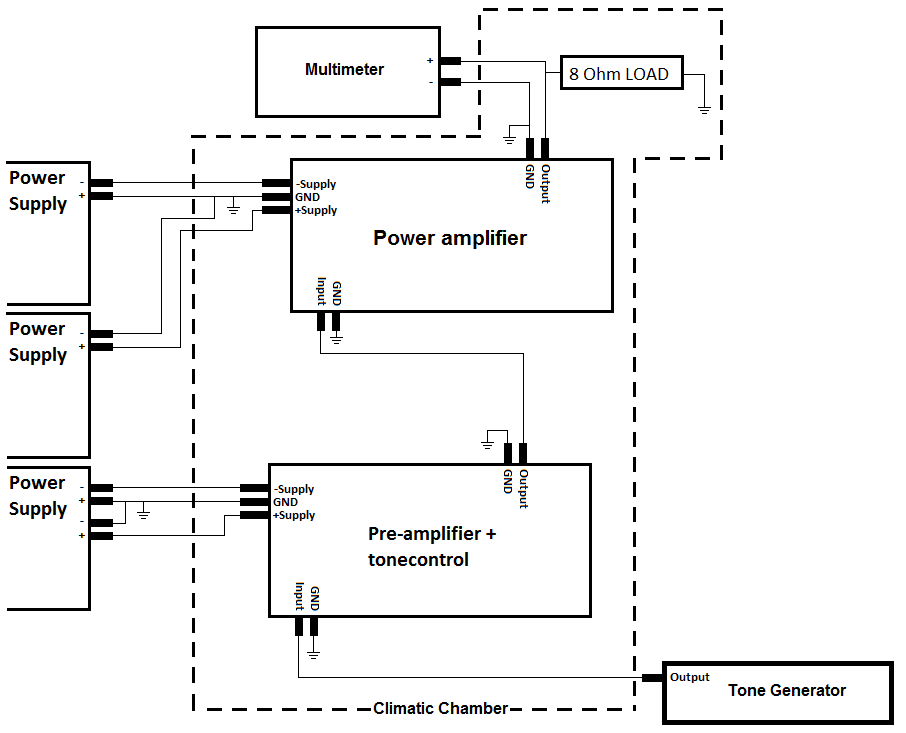
\includegraphics[scale=.8]{figures/filename}
	\flushleft
	\textit{SOURCE}
\end{figure}

%--------- NOTES ------------------------------------------------------
%Fxnotes wont compile properly inside the figure, only in the caption.
%Filetype can be specified but isn't needed.

\noindent
\figref{LABEL}\\

\noindent
\Figref{LABEL}

\vspace{.5cm}
%Do not use \vspace{length} or \hspace{length} unless exceedingly necessary.

%--------- BIBLIOGRAPHY REF EKSAMPLE -----------------------------------
This reference only represents this line since it is before the punctuation mark\cite{YDing}. This next reference however represents the entire section. That is all of the preceding sentences in the entire section. This is due to the fact that it is now after the punctuation mark in the end of the section (this is not used in the middle of a section!).\cite{YDing}
%>>>>>>>>>>>>>>>PLEASE ALSO READ THE NOTE IN myBib.bib<<<<<<<<<<<<<<<<<<
\pagebreak	%||||||||
%	\section{Table Sample}

\begin{table}[H]
\caption{This Is a Table\label{LABEL}}
\begin{tabular}{|l|p{5cm}|l|l|l|}
  \hline
  \textbf{No.}&\textbf{Description}&\textbf{Min}&\textbf{Max}&\textbf{Requirements}\\
  \hline
  1 & Some Text & Some Text & Some Text & Some Text\\
    &           &           &           & Some More Text\\
    &           &           &           & Text Text\\
    &           &           &           & Text Text Text\\
  \hline
  2 & Some Text & Some Text & Some Text & Some Text\\
  \hline
  3 & 	By specifying the width of a column (|p\{5cm\}|) the cells
  		in that column will will not exceed	the specified width    %Enter is used only for clarity and will not affect the compiled output.
  		but instead expand downward.
  		
  		        & Some Text & Some Text & Some Text\\
  \hline
  4 & Some Text & Some Text & Some Text & Some Text\\
  \hline
  \multicolumn{2}{|l|}{Some Text} 	&	\multicolumn{3}{l|}{Some Text}\\
  \hline
  \multicolumn{2}{|l|}{Text Text} 	&	\multicolumn{3}{l|}{Text = Text}\\
  \multicolumn{2}{|l|}{}			&	\multicolumn{3}{l|}{Text = Text}\\
  \multicolumn{2}{|l|}{}			&	\multicolumn{3}{l|}{Text = Text}\\
  \multicolumn{2}{|l|}{}			&	\multicolumn{3}{l|}{Text = Text}\\
  \multicolumn{2}{|l|}{}			&	\multicolumn{3}{l|}{Text = Text}\\
  \hline
  \multicolumn{2}{|l|}{Some Text} 	&	\multicolumn{3}{l|}{Teeeexxtt}\\
  \multicolumn{2}{|l|}{}			&	\multicolumn{3}{l|}{\LaTeX}\\
  \hline      
\end{tabular}
\end{table}

\noindent
\tableref{LABEL}\\

\noindent
\Tableref{LABEL}

\pagebreak	%||||||||
%	\section{Equation Sample}

\noindent
Some explanation:
%
\begin{align}
\unit{Unit}
[Equation]&=[Number]
\label{eq1}
\end{align}

\noindent
Some other explanation:
%
\begin{align}
\unit{Unit}
[Equation]&=[Number]
\label{eq2}
\end{align}

\noindent
Yet an explanation:
%
\begin{align}
\unit{Unit}
\text{You see? } [Equation]&=[Number]
\label{eq3}\\
%
\unit{Unit}
\text{Unit isn't aligned } \textbf{:( } \: [Equation]&=[Number]
\label{eq4}	   %
\end{align}	 	%
			  	 %
\noindent	   	  %
Explanation!:	   %
%				 	%
\begin{align}	  	 %
\unit{Unit}		   	  %
[Equation]&=[Number]   %	%-----------------------NOTES-----------------------%
\label{eq5}\\		 	%	% The &-sign aligns the equal signs.				%
%					  	 %	%													%
\unit{Unit}			   	  % % \unit{} will not be alligned by default,			%
[Equation]&=[Number]	   %% however the macro can be modded as described 		%
\label{eq6}\\			    % in macros.tex. This will allign the units,		%
%						    % but generate errors.								%
\unit{Unit}				    %													%
[Equation]&=[Number]		% \noindent should generally be used befor			%
\label{eq7}					% oneliners after equations, figures and tables.	%
\end{align}					%---------------------------------------------------%
\\
%
\noindent
\eqref{eq1}\\
\noindent
\eqrefTwo{eq1}{eq2}\\
\noindent
\eqrefThree{eq1}{eq2}{eq3}\\
\noindent
\eqrefFour{eq1}{eq2}{eq3}{eq4}\\
\noindent
\eqrefFive{eq1}{eq2}{eq3}{eq4}{eq5}\\
\noindent
\eqrefSix{eq1}{eq2}{eq3}{eq4}{eq5}{eq6}\\
\noindent
\eqrefSeven{eq1}{eq2}{eq3}{eq4}{eq5}{eq6}{eq7}\\
\noindent
\Eqref{eq1}\\
\noindent
\EqrefTwo{eq1}{eq2}\\
\noindent
\EqrefThree{eq1}{eq2}{eq3}\\
\noindent
\EqrefFour{eq1}{eq2}{eq3}{eq4}\\
\noindent
\EqrefFive{eq1}{eq2}{eq3}{eq4}{eq5}\\
\noindent
\EqrefSix{eq1}{eq2}{eq3}{eq4}{eq5}{eq6}\\
\noindent
\EqrefSeven{eq1}{eq2}{eq3}{eq4}{eq5}{eq6}{eq7}
\pagebreak	%||||||||
%|||||||												 ||||||||
%||||||||||||||||||||||||||||||||||||||||||||||||||||||||||||||||
%||||||||||||||||||||||||||||||||||||||||||||||||||||||||||||||||


%---------------------------INPUTS-------------------------------

\title{\Huge System til detektering af kropsbalance}
\author{\Large %Cecilie Topp, \\
Cecilie Sophie Rosenkrantz Topp \\ \Large Mads Jozwiak Pedersen \\ \Large Maria Kaalund Kroustrup \\ \Large Mathias Vassard Olsen \\ \Large Nikoline Suhr Kristensen \\ \Large Sofie Helene Bjørsrud Jensen \\
	\normalsize Sundhedsteknologi 3. semester\\
	\normalsize Aalborg univertsitet}
%\date{28. November 2014}
\maketitle
\vfill % Så sætter den det nedenunder i bunden af siden.

%\begin{abstract}
	%\begin{center}
		%her kan man måske skrive noget klogt 
	%\end{center}
%\end{abstract}
\clearpage

\tableofcontents
\clearpage

\chapter{Problemanalyse}
\section{Apopleksi}

Et apopleksi tilfælde kan være forårsaget af enten en blodprop i hjernen (iskæmisk) eller hjerneblødning (hæmoragisk).
Apopleksi er af World Health Organization (WHO) defineret som pludseligt opstået fokale neurologiske symptomer pga. forstyrrelser i hjernens blodcirkulation, der varer mere end 24 timer eller fører til døden[1]. Hvis varigheden er under 24 timer, betegnes det som transitorisk cerebral iskæmi (TCI), hvor de fleste tilfælde varer under 1 time[2] uden permanent hjerneskade [3].

(Billeder)

Iskæmisk apopleksi forekommer hyppigst%ift. hvad? 
[2] og opstår, når en hjernearterie blokeres af en blodprop (infarkt), der stopper tilførslen af blod til et bestemt område i hjernen, hvilket ses på figur xx. Infarkterne dannes primært pga. åreforkalkning enten ved en trombe, der dannes på stedet, eller emboli fra hjertet. Nervecellerne skades efter få minutter pga. stoppet blodtilførsel og vil gå tabt [5].

Hæmoragisk apopleksi skyldes hovedsageligt forhøjet blodtryk eller i sjældnere tilfælde bristede svagheder på arterier (aneurismer) eller misdannede kar[5]. Hæmoragisk apopleksi opstår, når en hjernearterie brister og lækage af blod danner en blodansamling (hæmatom), der beskadiger det omkringliggende væv og forøger trykket i hjernen, hvilket ses på figur xx. Blødning i selve hjernen (intracerebral hæmoragi) kommer af forhøjet blodtryk, der danner et pres på de små arterier, som får dem til at briste[4] og forekommer i 10-12\% af tilfældene[2]. %ift. hvilke tilfælde? 
Blødning i rummet mellem de to hjernehinder (subaraknoidalrummet) skyldes bristning af et aneurisme på en pulsåre i hjernen [5] og forekommer 3-5\% af tilfældene[2]. Symptomerne ved subaraknoidalblødning er generel tab af hjernefunktion, da der forekommer et øget pres på hjerneskallen, hvorimod ved intracerebral hæmoragi er hæmatomet lokaliseret et bestemt sted i hjernen og forårsager nedsat funktion ved én bestemt hjernefunktion[4]. 

% WHO - find en dansk difination istedet.
% Fjern paranteserne - skrev enten det rigtige ord først eller lav en anden måde at skrive det på.
% Mangler lidt en forklaring på, hvordan og hvorfor apopleksi det opstår. Man kan godt uddybe mere i det, der allerede er skrevet.
% Når der er bygget mere på, kan man godt lave nogle forskellige overskrifter.
% Fakta omkring, hvad der er årsagen til apopleksi - hjertesagen har nogle forksellige info om det. Fakta om apopleksi.
% !TeX spellcheck = da_DK
\section{Diagnosticering}

Når en patient med apopleksi indlægges, er grundig undersøgelse nødvendig for at identificere, hvilken form for apopleksi der er tale om. Dette trin er afgørende for det efterfølgende forløb, da behandling samt rehabilitering planlægges herefter. \cite{Sundhedsstyrelsen2009}

\subsection{Anamnese}
For at blive bekendt med patientens egen subjektive vurdering af det hidtidige sygdomsforløb, optager lægen en anamnese. Her skal sygdomsforløbet  beskrives detaljeret, og der skal desuden spørges ind til faktorer, som kan have været medvirkende til udviklingen af apopleksi såsom livsstil og sygdomme, herunder f.eks. diabetes og hjerteproblemer. \cite{Sundhedsstyrelsen2009}

\subsection{Klinisk undersøgelse}
Den kliniske undersøgelse udføres for at vurdere hvor alvorligt et sygdomstilfælde, der er tale om. Undersøgelsen udføres ud fra en standardiseret skala, da dette gør det muligt for andre læger at undersøge patienten på samme måde senere i forløbet. Resultatet af undersøgelsen er en samlet score udregnet fra resultatet af de enkelte undersøgelser. Det er således muligt at vurdere om der sker fremskridt hver gang undersøgelsen foretages. \cite{Sundhedsstyrelsen2009}

Der findes flere forskellige skalaer, som lægen kan anvende til at foretage den kliniske undersøgelse, herunder Scandinavian Stroke Scale, European Stroke Scale og Hemisperic Stroke Scale. Fælles for skalaerne er, at de alle undersøger både bevidsthedsniveau samt motoriske og kognitive egenskaber hos patienten \cite{Center, Centera, Centerb, Centerc}. I den danske sundhedssektor benyttes Scandinavian Stroke Scale, dette blev besluttet i Det Nationale Indikatorprojekt for apopleksi \cite{Apopleksi2009}. F.eks. har Region Syddanmark derudover forskellige retningslinjer for hvilken skala, der skal benyttes i et apopleksi forløb \cite{Syddanmark}. Alle apopleksi patienter, der bliver indlagt med mulig akut apopleksi eller TCI, skal have en score på Scandinavian Stroke Scale. Herefter benyttes National Institute of Health Stroke Scale hvis patienten skal have trombolysebehandling. Barthel Scale anvendes hvis patienten sendes til videre rehabilitering og beskriver patientens funktionsniveau i forhold til almindelige dagligdags funktioner. Til sidst benyttes Modificeret Rankin Scale til at give en beskrivelse af graden af handicap. \cite{Syddanmark}

\subsection{Videre undersøgelser}
Ved den videre undersøgelse vil der udføres en scanning for at undersøge, om patienten er ramt af en hjerneblødning eller en blodprop. Scanningen laves desuden for at lokalisere det ramte område. Enten udføres der en scanning af typen CT eller MR afhængigt af, hvad der er mest hensigtsmæssigt i den givne situation. \cite{Sundhedsstyrelsen2009} %CT-scanning udsender røntgenstråligen, hvilket optages i vævet på forskellige måder. Udfra dette beregner en computer tværsnitsbilleder af kroppens indre \fxnote{https://www.cancer.dk/hjaelp-viden/undersoegelser-for-kraeft/scanninger-billedundersoegelser/ct-scanning/}. Modsat anvendes der ved MR-scanning et kraftigt magnetfelt som sender radiobølger ind i kroppen. Derved registres et ekko og computeren kan derefter beregne et detaljeret billede af kroppens indre organer. 
CT-scanning anvendes f.eks. til undersøgelse af åreforkalkning og indre blødninger, hvor MR-scanning bruges til at undersøge sygdomme i nervesystemet f.eks. i hjernen \cite{Hansen2015,Ammundsen2015}.\\
Det skal derfor vurderes, hvilken form for scanning der skal anvendes ud fra forskellige kriterier, herunder lægens mistanke om, hvilket område af hjernen der er ramt, samt hvor længe symptomerne på apopleksi har optrådt. I visse tilfælde kan lægen vælge at anvende begge scanningstyper.  
Derudover skal patientens blodtryk måles jævnligt i den akutte fase for at sikre, at det falder gradvist til et normalt niveau i løbet af nogle timer til et døgn. Hvis blodtrykket pludselig falder meget, kan dette være et udtryk for en blodprop i hjertet. Det er derfor afgørende at følge udviklingen med jævnlige blodtryksmålinger. \cite{Sundhedsstyrelsen2009}
\\
Under forløbet bør andre faktorer også kontrolleres, herunder lungefunktion, blodsukker og kropstemperatur. Disse faktorer kan enten give information om apopleksien, eller de kan være væsentlige for patientens fremtidsprognoser og følger efter sygdomsforløbet. \cite{Sundhedsstyrelsen2009}
\\

% [1] Sundhedsstyrelsens rapport
% [2]http://www.strokecenter.org/professionals/stroke-diagnosis/stroke-assessment-scales/
% [3]http://www.strokecenter.org/wp-content/uploads/2011/08/hemispheric.pdf
% [4]http://www.strokecenter.org/wp-content/uploads/2011/08/scandinavian.pdf
% [5]http://www.strokecenter.org/wp-content/uploads/2011/08/European_Stroke_Scale.pdf
% [6]http://www.dsks.dk/filer/hoeringssvar/referenceprogram_for_behandling_af_patienter_med_apopleksi.pdf
% [7] http://ekstern.infonet.regionsyddanmark.dk/Files/dokument90214.htm
% [8] https://www.sundhed.dk/borger/sygdomme-a-aa/hjerte-og-blodkar/sygdomme/apopleksi/apopleksi-blodprop-eller-bloedning-i-hjernen/
% [9] http://academic.eb.com.zorac.aub.aau.dk/EBchecked/topic/569347/stroke
% [10] http://www.netdoktor.dk/sygdomme/fakta/blodprophjerne.htm
\input{rapportAfsnit/cProblemanalyse/Foelger}
\section{Samfundsmæssige omkostninger}
I Danmark opstår 12.000 tilfælde af apopleksi årligt. Apopleksi er den sygdom, hvor der kræves flest plejedøgn i sundhedssektoren [1]. %Uddyb - hvad er et plejedøgn, hvor mange kræver andre syge ?
Omkostningerne for patienter med følger af apopleksi har både direkte og indirekte omkostninger. De direkte omkostninger er udgifter til medicinering, sundhedsomkostninger i form af behandling i hospitalsvæsnet, praktiserende læge og speciallæge, samt hospitalsindlæggelse og rehabilitering både fra et samfundsmæssigt, regionalt og kommunalt perspektiv[2]. De indirekte omkostninger  består af udgifter for tabt arbejdsfortjeneste, tabt produktivitet og ekspertise for samfundet som følge af fravær, tidsforbrug, fremtidige relaterende omkostninger og sundhedsomkostninger til personer med hjerneskade ved forlænget levetid[2].

\subsection{Samlede omkostnigner}
De samlede sundhedsomkostninger i 2008 var 110.000 kroner, hvilket inkluderer incidens-år og året efter. Omkostninger uden for sundhedssektoren, dvs. kommunal rehabilitering ligger på omkring 60.00 kroner pr. patientforløb. I følge sundhedsstyrelsen bærer kommunen ca. 35\% af de offentlige konsekvenser af hjerneskade og hjerneskaderehabilitering rent økonomisk. [2]    
Alt efter sværhedsgraden af hjerneskaden kan produktivitetstab forekomme hos patienten. Dette betyder, at patienterne som rammes af apopleksi i nogle tilfældes er nødsaget til at modtage indkomsterstattende ydelser, såsom arbejdsløshedspenge, sygedagpenge, førtidspension, efterløn osv. En del af patienterne er dog allerede på indkomsterstattende ydelser i form af pension, da alders gennemsnittet for patienter med hjerneskade er gennemsnitlig 62,4 år. Produktivitetstabet formodes at koste samfundet 50.000 kroner årligt, hvilket er beregnet ud fra populationen fra 2004. 

I alt vil omkostningerne for hjerneskaderehabilitering og rehabilitering være 270.000 kroner i en to-årig periode bereget ud fra tal fra 2008[2]. De samlede udgifter for patienter med apopleksi udgør 4\% af sundhedsvæsenets samlede udgifter, her direkte udgifter estimeret til 2.7 milliard kroner om året[3]. 
Patienter med apopleksi er altså omkostningsfuld for samfundet, da der som tidligere nævnt blandt andet kræves en del plejedøgn på grund af funktionsnedsættelse, samt udgifter til rehabilitering og pruduktivitetstab.

\section{Organisatorisk}
I sundhedssektoren arbejder de forskellige dele af organisationen på tværs af hinanden, så der skal være et samarbejde mellem syghuse, kommuner og praktiserende læger. Dette samarbejde skal ske både internt på syghusene, på afdelingerne og kommunalt mellem forvaltningerne [2]. Dette sammenspil mellem de ovennævnte aktører er vigtigt, da hjerneskadede berører flere afdelinger og derfor har brug for involvering af flere sundhedsprofessionelle grupper under sin behandling og rehabilitering på grund af de omfattende og alvorlige konsekvenser.

De ovennævnte aktører er de organisatoriske enheder, der har en central rolle i forløbet. Det er ikke muligt at fastlægge en egentlig organisering af hjerneskaderehabiliteringen i Danmark, da sammenspillet mellem de forskellige aktører er meget flydende og forskellige alt efter hvor i landet man befinder sig og hvor omfattende hjerneskaden er. Denne forskel opleves regionalt, hvor behandling og rehabilitering enkelte steder foregår på få af sygehusets afdelinger, mens patienter andre steder behandles på et rehabiliteringssygehus, efter den akutte behandling er foretaget[2]. 

I starten af behandlingssforløbet sendes patienterne til neurologiske, geriatriske, neurokirurgiske og medicinske afdelinger på sygehuset[2]. Som tidligere nævnt inddeles patienterne efter sværhedsgrad af hjerneskaden, hvor de sværest ramte, som er patienter med traumatisk hjerneskade og tilgrænsede lidelser, henvendes til Hammel og Hvidovre. Rehabiliteringen kan også ske på rehabiliteringsafsnittet på sygehusene i dele af landet[2].
Det primære ansvar ligger hos kommunerne i form af genoptræningsplanens afdækning af rehabiliteringsbehov, dvs. at kommunerne holder øje med om dette foregår i praksis, herunder bl.a. patientens genoptræningsbehov. Kommunerne har derudover mulighed for at henvise patienterne til egne tilbud, eller henvise til private[2]. 

Afslutningsvis gennemgår patienterne et langt og forskelligt behandlingsforløb alt efter hvilken grad hjerneskaden er, som indebærer et samarbejde mellem de forskellige aktører. Efter behandlingen står, som nævnt før, kommunerne for det primære ansvar i forhold til rehabilitering og henvisning for patienten.
  

%[1]https://www.sundhed.dk/borger/sygdomme-a-aa/hjerte-og-blodkar/sygdomme/apopleksi/apopleksi-blodprop-eller-bloedning-i-hjernen/
%[2]http://sundhedsstyrelsen.dk/~/media/CB8CCFE77832456C8B1BABF2F558A661.ashx
%[3]http://www.hjernesagen.dk/om-hjerneskader/bloedning-eller-blodprop-i-hjernen/fakta-om-apopleksi


%%%%% Nye opgaver:
% Evt lave en tabel over tallene i afsnittet.


%%%%%%%%%%%%%%%%%% Udkommenteret
% (slet) Hvis der ses på omkostninger for de samlede hjerneskadede, vil omkostningerne for en patient efter hjerneskaden indtræden på en 5 årig periode fra 2005-2009 ligge på sundhedsomkostninger for gennemsnitlig 27.200 kroner i aldersgruppen 18+. Det er vanskeligt at vurdere, hvilken betydning denne omkostningen vil have, da omkostningerne er beregnet som en sum af Diagnose Relaterede Grupper(DRG)-omkostninger, hvilket vil sige at omkostningerne er opgjort efter forskellige takstsystemer [2].
% (slet) Ligeledes er der ikke en konkret overgang fra indlæggelse til påbegyndelse af rehabiliteringsforløbet, da rehabiliteringen forekommer ved indlæggelse (%og derved har en glidende overgang). Den samlede overgang omtales hjerneskaderehabilitering %(forstår ikke helt, hvad der menes med samlede overgang). Det antages, at de kommunale omkostninger ligger gennemsnitlig på 60.000 kr. pr. forløb regnet i 2008-prisniveau [2]. Derudover er der de første to år af behandingsomkostninger i forhold til hjernebehandlings- og rehabiliteringsforløbet en omkostning på 110.000 kr. [2].
%I sundhedssektoren arbejder de forskellige dele af organisationen på tværs af hinanden, hvilket vil sige, at der skal være et samarbejde mellem sygehuse, kommuner og praktiserende læger. Dette samarbejde skal ske både internt på sygehusene, afdelingerne i mellem og kommunalt, mellem forvaltningerne [2]. Dette sammenspil mellem de ovennævnte aktører er vigtigt, da hjerneskadede kræver involvering af flere sundhedsprofessionelle grupper, da der er omfattende og alvorlige konsekvenser ved tilfælde af apopleksi for både patienter, så vel som for pårørende. 
%Patienterne sendes som regel til den første del af behandlingen hos neurologiske, geriatriske, neurokirurgiske og medicinske afdelinger på sygehuset[2]. Som tidligere nævnt inddeles patienterne efter sværhedsgrad af hjerneskaden, hvor de sværest ramte, som er patienter med traumatisk hjerneskade og tilgrænsede lidelser, henvendes til Hammel og Hvidovre. Rehabiliteringen kan også ske på rehabiliteringsafsnittet på sygehusene i dele af landet[2]. 
%Patienter som får en hjerneskade er omkostningsfuld for samfundet, da der som tidligere nævnt bl.a. kræves en del plejedøgn, da patienterne vil have alvorlige følger som vil kunne forårsage nedsat livsfunktioner. Dette vil foruden behandling kræve rehabilitering og kunne medfører produktivitetstab, hvilket yderligere kan være en omkostning, hvis patienterne har følger af hjerneskaden på længere sigt.
%Der vil dog være en del af patienterne som i forvejen er på indkomsterstattende ydelser (findes der ikke et andet ord for det?) i form af pension, hvilket afspejles i at alders gennemsnittet for patienter med hjerneskade er 62,4 år[2]. Produktivitivtetstabet vil for en hjerneskadet patient i det samlede koste samfundet 50.000 kr. årligt, for de første seks år regnet i 2008-prisniveau[2]. 
% (kan det evt. slettes??) Omkostningerne for både den primære sektor dvs. kommunen og sygehusomkostningerne forskellige. Rehabiliteringen vil for den primære sektor i gennemsnit ligge på 600 kr i perioden 2008-2009 og inden for sygehusomkostninger på 3.200 kr i samme periode, begge for patienter med hjerneskade beregnet i 2008-prisniveau [2].
% mangler en forklaring på, hvad den sekundære sektor er.
% Gøre det mere synligt at behandlingerne er forskellige imellem kommunerne - jeg synes altså det er beskrevet ok i afsnittet over. Så skal man skrive sådan noget som "som nævn ovenfor" - hvilket virker mærkeligt.
%Patienter vil skulle gennemgå et langt og forskelligt forløb alt efter hvilken grad hjerneskaden har været, dette indebærer et samarbejde mellem de forskellige aktører, som har en flydende overgang mellem hinanden. Efter behandlingen på de forskellige afdelinger og sygehus står, som tidligere nævnt, kommunerne for den primære ansvar i forhold til rehabiliteringen og henvisninger for patienten.
\section{Rehabilitering}
Når selve slagtilfældet er stabiliseret og behandlet, er det essentielt, at rehabiliteringen af en apopleksipatient indfindes hurtigst muligt - gerne 1 til 2 dage efter slagtilfældet. I Danmark dækker rehabilitering af en patient med apopleksi områderne: direkte træning af funktioner, reorganisering af netværk (ufrivilligt - hjernens proces), kompenserende strategier, ændringer i miljø, social og psykologisk støtte. Genoptræningen omhandler dog ikke kun træning med en ergo- eller fysioterapeut, da plejepersonale til dagens almindelige gøremål også essentiel. Patientens daglige rutiner kan være gået tabt under slagtilfældet, hvorfor det er vigtigt, at få patienten tilbage i sit vante miljø. Plejepersonale skal hjælpe patienten til at genfinde denne rytme og hjælpe patienten til eventuelt at udføre dagligdags ting på en ny måde. Det kan ske, at patienten ikke længere er i stand til at beherske begge sine hænder til en opgave, hvorved plejepersonalet skal bistå patienten i indlæringen af kun at benytte en hånd. \\ 
Motoriske og sensoriske funktionsproblemer kan lede til balancebesvær for patienten i både siddende, stående og gående stilling. Der er afprøvet adskillige farmakologiske midler og behandlingsstadegier for at forbedre hjernens rehabilitering og motoriske funktioner. F.eks. er der afprøvet, at tildele apopleksipatienter det antidepressive middel Prozac (fluoxetin) i kombination med fysioterapi. Derudover er kortikal stimulation afprøvet, hvor området af hjernen, som kontrollerer motorstyring, modtager elektriske impulser fra en implanteret anordning. Denne mulighed har haft blandede succesoplevelser, men er udelukkende afprøvet på patienter, der har oplevet et alvorligt slagtilfælde. \cite{Academic2015} \\  
Apopleksi patienten skal i samarbejde med lægen, sygeplejersken og andet hjælpepersonale opstille nogle mål for sin rehabilitering. Målene skal hverken være for svære eller for lette, så patienten ikke mister sin motivation til genoptræningen. \cite{Kruuse2015} \\ 

\subsection{Forløbsprogram for rehabilitering} 
Sundhedsstyrelsen har udarbejdet et forløbsprogram for rehabilitering af patienter med erhvervet hjerneskade. Forløbsprogrammet strækker sig fra at patienten erhverver hjerneskaden til at patienten har opnået bedst mulig funktionsevne, hvorefter der udføres kontrol og vedligeholdelse af funktionsevnen. Tidsperioden af rehabilitering varierer ift. hjerneskadens sværhedsgrad, samt sværhedsgraden af funktionstabet. %dog kan perioden vare flere år.  
\cite{Sundhedsstyrelsen2011a} \\
Forløbsprogrammet er essentielt ift. at kunne give patienten den korrekte rehabilitering. Patienterne har forskellige behov og er afhængighed af hjælp fra plejepersonale samt forskellige former for teknologier i de forskellige faser. Det vil derfor være oplagt at undersøge, hvilken form for rehabilitering der er at foretrække i de enkelte faser.

\subsubsection{De tre faser i forløbsprogrammet}
\begin{figure}[H]
	\centering
	\includegraphics[scale=0.8]{figures/bProblemanalyse/flowdiagram_faser1.png}
	\caption{På figuren ses et overblik over de 3 faser som patienter med apopleksi skal igennem i forløbsprogrammet for rehabilitering. Figuren er lavet på baggrund af sundhedsstyrelsen.\cite{Sundhedsstyrelsen2011a}} \fxnote{ved ikke om vi skal bruge dette som kilde når vi selv har udarbejdet den - om det så er nok at skrive det i teksten.}
	\label{tre_faser}
\end{figure}

Den første fase, som ses på \ref{tre_faser} afspejler forløbsprogrammet som foregår på sygehusets apopleksiafdeling. På apopleksiafdelingen fortages primært akut behandling for at begrænse skaderne. Når patientens sikkerhed er sikret og skaderne er begrænset påbegyndes den tidlige rehabilitering. Under den tidlige rehabilitering giver en speciallæge i neurologi en vurdering af patientens rehabiliteringsbehov. Derudover bliver patienterne overvåget ift. bevidsthed, ændringer og amnesi samt foretaget vurderinger af basale fysiologiske funktioner, samt iværksat træning i diverse bevægelsesfunktioner, basale egenskaber og kommunikationsfunktioner. Patienterne gennemgår også en tidlig behandling og diagnostik for at undersøge komplicerende tilstande, som f.eks. vaskulære hændelser, blodpropper i ben og lunger, smerte, sansefunktioner og adfærdsfunktioner. Patienterne vurderes i denne fase af fagkyndigt personale som ergoterapeut, fysioterapeut og audiologopæd. Disse er med til, at sikre, at patienten udfører træningen korrekt ift. stilmulering og træning af bevægelsesfunktioner, taletræning og udførsel af basale daglige aktiviteter.\cite{Sundhedsstyrelsen2011a} \\

I den anden fase, hvilket fremgår af \ref{tre_faser}, gennemgår patienten rehabilitering på sygehuset, hvor der er fokus på de skadede funktioner, ligeledes bliver patienten på samme måde som i fase et undervist af fagkyndigt personale. Hvorefter patientens behov for rehabilitering og rehabiliteringens udvikling vurderes. Patienterne bliver i denne fase udredet ift. funktionsevne, mentale funktioner, bevægelsesfunktioner herunder bevægelse og mobilitet i led, knogler, reflekser og muskler samt   rehabilitering med henblik på daglige aktiviteter. Hvis patienten vurderes til at have en stabil udvikling i rehabiliteringsprocessen, vil patienten blive udskrevet og påbegynde fase tre. \cite{Sundhedsstyrelsen2011a} \\


I den tredje fase er patienten udskrevet fra sygehuset, og derved forgår rehabilitering som ambulant rehabilitering og selvstændig træning, dette fremgår af \ref{tre_faser}. Hvorvidt patienten skal vedblive rehabilitering på sygehuset, eller om patienten henvises til rehabilitering i de kommunale rehabiliteringscentre afgøres på baggrund af observationer foretaget i anden fase. Derudover afgøres det om enkelte rehabiliteringer fra anden fase skal igangsættes eller fortsætte. Den selvstændige træningen, kan for patienterne med neglekt være en udfordring ift. bevægelsesmønstre og kropsholdning, da de kan have problemer med balancen og opmærksomheden på kroppen. Patienterne går derfor stadig til kontrol og vedligeholdelse for at sikre, at rehabiliteringens udvikling er stabil. Det kan i sidste ende have betydning for, hvor lang tid det tager for patienten at generhverve sine tabte funktioner. Den tredje fase varierer derfor fra patient til patient alt efter udviklingen af rehabiliteringen.\cite{Sundhedsstyrelsen2011a}



% I første og anden fase af rehabiliteringsforløbet bliver patienten undervist og overvåget af fagkyndigt personale. Dette gøres for at sikre, at patienten udfører træningen korrekt f.eks. med bevægelsesmønstre, og korrigere patienten til at bevægelsen og øvelserne udføres korrekt. Dette er vigtigt, da patienten, som sagt i tredje fase, selv skal foretage den nødvendige træning og dermed har fornemmelse af, hvordan træningen udføres korrekt ift. bevægelsesmønstre og kropsholdning. Dette kan midlertidig være en udfordring for apopleksipatienter med neglekt, da de kan have problemer med balancen og opmærksomheden på kroppen. Patienten går derfor stadig til kontrol og vedligeholdelse for at sikre, at rehabiliteringens udvikling er stabil. Det kan i sidste ende have betydning for, hvor lang tid det tager for patienten at generhverve sine tabte funktioner. Den tredje fase varierer derfor fra patient til patient alt efter udviklingen på rehabiliteringen. \cite{Sundhedsstyrelsen2011a}

\section{Biofeedback}
Biofeedback teknologien blev introduceret i slutningen af 1960. Denne teknologi gør det muligt for en patient at opnå bevidst kontrol over latent nervefunktion, samt forbedre rehabiliteringen. Dette sker ved et auditiv eller visuel tegn på, at deres bevægelse har aktiveret en neuromuskulær genvej. Biofeedback teknologien har bla. haft stor succes i behandling af apopleksi patienter med fækal- og urin inkontinens. Biofeedback kan også være gavnligt for en apopleksipatient med balanceproblemer, herunder pusher-syndrom forårsaget af følelsesløshed i den ene side af kroppen. Patienten har stadigvæk kontakt til hele sin krop, men kan ikke fornemme den ene halvdel. Hvis patienten underrettes om, at han/hun har forkert kropsholdning, som vil lede til mistet balance, kan patienten pga. et signal nå at rette op på dette, inden et uheld indtræffer. \\ 

Hvis en patient skal have gavn af biofeedback teknologien kræver det, at patienten har en kognitiv kapacitet til at følge instruktionerne under behandlingssessioner og fastholde læring fra session til session. Derudover kræves en neurologiske kapacitet til at genskabe frivillig kontrol. \cite{Middaugh1989} \\
 
Der findes apparater og sensorer til at opfange et fysiologisk signal, der kan bruges til bevægelses-, styrke- og balancetræning, og som afgiver et biofeedback tilbage til patienten. Der findes f.eks. et hånd dynamometer, der kan benyttes til at måle styrkeforskellen i hhv. højre og venstre hånd. Dette kan være fordelagtigt at benytte for en apopleksipatient med balanceproblemer, herunder eksempelvis pusher-syndrom, da patienten derved gøres opmærksom på styrken i sin følelsesløse side. Herudover findes et smerte algometer, som kan gemme målinger af smerte, en trykplade, som kan måle fordelingen af en persons kropsvægt under forskellige øvelser, gyroskop, som kan måle accelerationen i en bestemt retning, accelerometer, som kan måle kropshældning, når sensoren er placeret på patienten, samt diverse elektroder, som f.eks. kan måle muskelaktivitet. Valget af hvilke apparater og sensorer der er fordelagtige afhænger af patientens tilstand f.eks. hørelse og følsomhed, samt sværhedsgraden af hjerneskaden og hvilke funktioner, der skal genoptrænes. \cite{Hjaelpemiddelbasen} %mangler en kilde på, hvad de forskellige gør. - skal vi ikke have dette i en tabel?

%\begin{table}[Biofeedback]
%\centering
%\caption{My caption}
%\label{my-label}
%\begin{tabular}{lllll}
%{\bf Apparatur}  & {\bf Funktion}                                                                                                                                                                                                                                         %&  &  &  \\
%Hånd dynamometer & Måler styrkeforskellen i hhv. højre og venstre hånd. Dette kan være fordelagtigt at benytte for en %apopleksipatient med balanceproblemer, herunder eksempelvis pusher-syndrom, da patienten derved gøres opmærksom på %styrken i sin følelsesløse side. &  &  &  \\
%Smerte algometer & Målinger af smerte, en trykplade, som kan måle fordelingen af en persons kropsvægt under %forskellige øvelser                                                                                                                                           %&  &  &  \\
%Gyroskop         & Måler accelerationen i en bestemt retning                                                                                                                                                                                                              %&  &  &  \\
%Accelerometer    & Måler kropshældning, når sensoren er placeret på patienten, samt diverse elektroder, som f.eks. kan måle muskelaktivitet                                                                                                                               &  &  & 
%\end{tabular}
%\end{table}


%[1] - http://academic.eb.com.zorac.aub.aau.dk/EBchecked/topic/569347/stroke
%[2] - https://www.sundhed.dk/borger/sygdomme-a-aa/hjerte-og-blodkar/sygdomme/apopleksi/		   apopleksi-rehabilitering/
%[3] - http://link.springer.com.zorac.aub.aau.dk/article/10.1007/BF00999338    http://www.archives-pmr.org/article/S0003-9993(95)80503-6/abstract
%[4] - http://www.hmi-basen.dk/r4x.asp?linktype=iso&linkinfo=044824&P=1              
%[5] - Sundhedsstyrelsen, 2011. Sundhedsstyrelsen. Forløbsprogram for rehabilitering af voksne med erhvervet hjerneskade. Sundhedstyrrelsen, 2011.


%\section{Rehabilitering}
%Når selve slagtilfældet er stabiliseret og behandlet, er det essentielt, at rehabiliteringen af en apopleksi patient indfindes hurtigst muligt - gerne 1 til 2 dage efter slagtilfældet. Rehabiliteringen kan indebære fysisk, erhvervsmæssig eller tale terapi. Motoriske og sensoriske funktionsproblemer kan lede til balancebesvær for patienten i både siddende, stående og gående stilling. Der er afprøvet adskillige farmakologiske midler og behandlingsstadegier for at forbedre hjernens rehabilitering og motoriske funktioner. F.eks. er der afprøvet, at tildele apopleksi patienter det antidepressive middel Prozac (fluoxetin) i kombination med fysioterapi. Derudover er kortikal stimulation afprøvet, hvor området af hjernen, som kontrollerer motorstyring, modtager elektriske impulser fra en implanteret anordning. Denne mulighed har haft blandede succes oplevelser, men er udelukkende blevet afprøvet på patienter, der har oplevet et alvorligt slagtilfælde. \\ %http://academic.eb.com.zorac.aub.aau.dk/EBchecked/topic/569347/stroke                             % Hvor foregår rehabiliteringen ift. hvor slemt det er?
%Genoptræningen af en apopleksi patient i Danmark dækker områderne direkte træning af funktioner, reorganisering af netværk (ufrivviligt - hjernens proces), kompenserende strategier, ændringer i miljø, social og psykologisk støtte. Genoptræningen omhandler dog ikke kun træning med en ergo- eller fysioterapeut, da plejepersonale til dagens almindelige gøremål også spiller en stor rolle. Patientens daglige rutiner kan være gået tabt under slagtilfældet, og det er derfor utrolig vigtigt at få patienten tilbage i sit vante miljø. Plejepersonale skal hjælpe patienten til at genfinde denne rytme og hjælpe patienten til eventuelt at udføre dagligdags ting på en ny måde. Det kan ske, at patienten ikke længere er i stand til at beherske begge sine hænder til en opgave, hvorved plejepersonalet skal bistå patienten i indlæringen af kun at benytte en hånd. \\
%Apopleksi patienten skal i samarbejde med lægen, sygeplejersken og andet hjælpepersonale opstille nogle mål for sin rehabilitering. Målene skal hverken være for svære eller for lette, så patienten ikke mister sin motivation til genoptræningen. \\ %https://www.sundhed.dk/borger/sygdomme-a-aa/hjerte-og-blodkar/sygdomme/apopleksi/apopleksi-rehabilitering/

%indledning nr. 2
%Når selve slagtilfældet er stabiliseret og behandlet, er det essentielt, at rehabiliteringen af en apopleksi patient indfindes hurtigst muligt - gerne 1 til 2 dage efter slagtilfældet. Rehabiliteringen kan indebære fysisk, erhvervsmæssig eller tale terapi. Motoriske og sensoriske funktionsproblemer kan lede til balancebesvær for patienten i både siddende, stående og gående stilling. Der er afprøvet adskillige farmakologiske midler og behandlingsstadegier for at forbedre hjernens rehabilitering og motoriske funktioner. F.eks. er der afprøvet, at tildele apopleksi patienter det antidepressive middel Prozac (fluoxetin) i kombination med fysioterapi. Derudover er kortikal stimulation afprøvet, hvor området af hjernen, som kontrollerer motorstyring, modtager elektriske impulser fra en implanteret anordning. Denne mulighed har haft blandede succes oplevelser, men er udelukkende blevet afprøvet på patienter, der har oplevet et alvorligt slagtilfælde. [1] \\    
                         
%Rehabiliteringen af en apopleksi patient i Danmark dækker områderne direkte træning af funktioner, reorganisering af netværk (ufrivilligt - hjernens proces), kompenserende strategier, ændringer i miljø, social og psykologisk støtte. Genoptræningen omhandler dog ikke kun træning med en ergo- eller fysioterapeut, da plejepersonale til dagens almindelige gøremål også spiller en stor rolle. Patientens daglige rutiner kan være gået tabt under slagtilfældet, og det er derfor utrolig vigtigt, at få patienten tilbage i sit vante miljø. Plejepersonale skal hjælpe patienten til at genfinde denne rytme og hjælpe patienten til eventuelt at udføre dagligdags ting på en ny måde. Det kan ske, at patienten ikke længere er i stand til at beherske begge sine hænder til en opgave, hvorved plejepersonalet skal bistå patienten i indlæringen af kun at benytte en hånd. \\ 

% Kan de to overstående afsnit skrives sammen, så man starter mere bredt og derefter indskærper sig. Båske bytte om på rækkefælgen i det præsenterede? Husk at lave det gamle stå, hvis man forsøger sig med en omformulering. - 

%\section{Biofeedback}
%Biofeedback teknologien blev introduceret i slutningen af 1960. Denne teknologi gør det muligt for en patient at opnå bevidst kontrol over en voluntær men latent nervefunktion. Dette sker ved en auditiv eller visuel tegn på, at deres bevægelse har aktiveret en neuromuskulær genvej. Biofeedback teknologien har bla. haft stor succes i behandling af apopleksi patienter med fækal- og urin inkontinens. Teknologien kunne også være gavnligt for en apopleksi patient, som har udviklet pusher-syndrom, da dette skaber balanceproblemer pga. følelsesløshed i den ene side af kroppen. Patienten har altså stadig kontakt til hele sin krop, men kan ikke fornemme den ene halvdel. Hvis patienten blev underrettet om, at han/hun havde forkert kropsholdning, som ville lede til at miste balancen, kunne patienten nå at rette op på dette, inden et uheld vil indtræffe. \\
%Hvis en patient skulle have gang af biofeedback teknologien kræver det dog, at patienten har en kognitive kapacitet til at følge instruktionerne under behandlings sessioner og fastholde læring fra session til session. Derudover kræves en neurologiske kapacitet til at genskabe frivillig kontrol. \\ %   http://link.springer.com.zorac.aub.aau.dk/article/10.1007/BF00999338    http://www.archives-pmr.org/article/S0003-9993(95)80503-6/abstract
%Der findes apparater på markedet til bevægelses-, styrke- og balancetræning, som afgiver et biofeedback til patienten. Der findes f.eks. et hånd dynamometer, som kan benyttes til at måle styrkeforskellen i henholdsvis højre og venstre hånd. Dette kan være fordelagtigt at benytte for en apopleksi patient, som har udviklet pusher-syndrom, da patienten derved bliver opmærksom på styrken i sin følelsesløse side. Herudover findes et smerte algometer, som kan gemme målinger af smerte. %http://www.hmi-basen.dk/r4x.asp?linktype=iso&linkinfo=044824&P=1               % Vurder, om det med hånddynamometer er "to far off" og skal slettes.

% Bruges det kun på latente nervefunktioner? Skal ændres lidt, så det ikke kun er latente nerfunktioner, der snakkes om i biofeedback afsnittet. Udbyg mere her.
% Udbyg de forskellige rehabiliteringstyper - undersøg og vurder, om der kan skrives mere på? Gerne med underoverskrifter.
% Hvordan fungerer rehabiliteringen der hjemme?
% Vi skal have fokus på, hvor vi gerne vil hen. Få strikket den røde tråd (balance) ind i teksten, så fokus kommer på det.
% Mangler et overblik over, hvor lang tid rehabiliteringen tager - nogle eksempler på, hvor lang tid rehabiliteringen kan tage.
% Biofeedback afsnittet er måske lidt for specifikt på pusher-syndrom. Skal muligvis skrives om, så det bliver mere generelt med fokus på balance.
% Hvordan skal man give biofeedback til en ældre person, hvis de har dårlig hørelse og følelelse?


\section{Indlæggelsesforløb og Personlige Omkostninger}
Indlæggelsesforløbene for apopleksipatienter varierer både i antal og hyppighed afhængig af forskellige faktorer - herunder alder og køn.

\subsection{Indlæggelsesforløb}
I 2010 var der i Danmark 18.041 indlæggelsesforløb forbundet med hjerneskade. Indlæggelsesforløbene kan inddeles i seks kategorier: Spontan blødning i hjernen, spontan infarkt i hjernen, uspecificeret apopleksi, diverse apopleksitilfælde, sequelae og TCI. \fxnote{Ydermere er forløbet for alle apopleksitilfælde inddelt i gruppe for sig selv, dette vil sige alle foruden sequelae og TCI.} Den hyppigste diagnose iblandt apopleksitilfælde var i 2010 spontan infarkt i hjernen med 6832 indlæggelsesforløb, hvilket svarer til omkring 38\% af alle forløbene. Den næsthyppigste var TCI som stod for omkring 27 \% af forløbene, hvor den laveste andel af indlæggelsesforløb, kaldet diverse, står for 0,8\% af det samlede antal. \fxnote{tænkte at vi kunne lave en tabel over de forskellige antal og sige at for yderligere kan ses i appendix, ellers kan vi sætte den ind} Indlæggelsesforløbene for apopleksi (ekslusiv sequale) er faldet siden år 2000, hvilket kan ses på \figref{Indlaeggelser}.\cite{Sundhedsstyrelsen2011}

\begin{figure}[H]
	\caption{Indlæggelsesforløb for apopleksi}
	\label{Indlaeggelser}
	\centering
	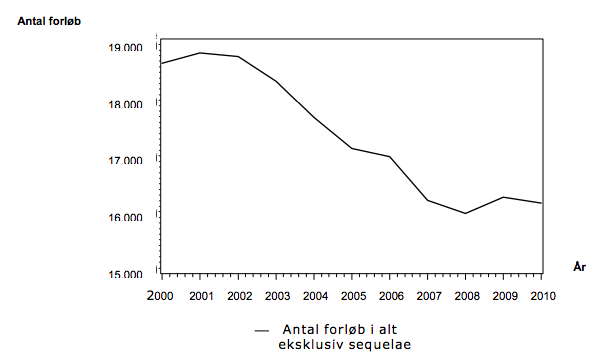
\includegraphics[scale=.5]{figures/bProblemanalyse/Figur1}
	\flushleft
	\textit{Her illustreres faldet i antallet af indlæggelsesforløb siden 2000.}
\end{figure}

Indlæggelsesforløbene har forskellig længde. 16.460 forløb, og dermed størstedelen, varede under 15 dage. For perioden fra 15-28 dage var der 1.191 forløb. Efter dette var tallet støt faldende, med kun 3 indlæggelsesforløb der er over 150 dage \cite{Sundhedsstyrelsen2011}.

\subsection{Køn- og aldersfordeling}
Hvis der ses på fordelingen af køn og aldersgrupper der rammes af apopleksi, stod mændene i 2010 for 9.710 af alle tilfælde, mens kvinderne stod for 8.562 \cite{Sundhedsstyrelsen2011}. Dette svarer til at mændene stod for 53\% af alle tilfældene\fxnote{mangler kilde}. Fordelingen kan ses på \figref{AlderKoen}.  
Antallet af indlæggelsesforløb for mænd stiger, når de bliver ældre end 65 år. Dette ses også på \figref{AlderKoen}, der viser at der i 2010 næsten skete en fordobling i gruppen 65+ i forhold til gruppen under 65.
Kvinders antal af indlæggelsesforløb fulgte samme mønster som mændene, og steg til over det dobbelte ved gruppen 65+ i forhold til gruppen under 65, som pgså er illustreret på \figref{AlderKoen}.\cite{Sundhedsstyrelsen2011} Alderen er således en væsentlig faktor for forekomsten af apopleksi.

\begin{figure}[H]
	\caption{Alders- og kønsfordeling}
	\label{AlderKoen}
	\centering
	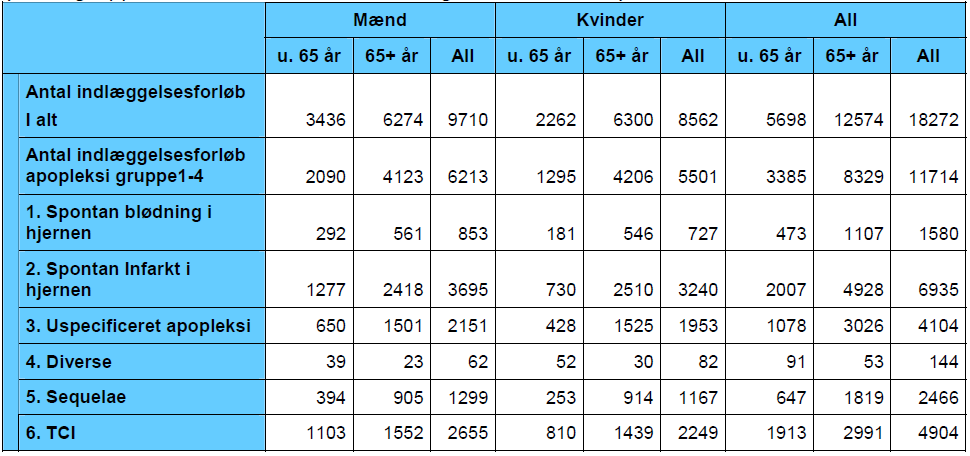
\includegraphics[scale=.8]{figures/bProblemanalyse/MaendKvinder}
	\flushleft
	\textit{Tabellen viser fordelingen af apopleksipatienter i forhold til alder og køn i 2010.}
\end{figure}

%\subsection{Fremtidsprognoser}
%Patienterne kan, som tidligere nævnt, rammes af en række følger som både kan have indflydelse på det fysiske og mentale. Ud fra alle tilfælde af apopleksi levede 75.000 over 18 i år 2011 med følger efter et slagstilfælde \cite{Hjernesagen2015}. Dette tal forventes at være stigende i takt med at der kommer flere ældre \cite{Sagen2014}. Antallet der dør af hjerneskader har været stagneret de sidste 10 år før 2011, hvor 14 \% døde inden for 30 dage \cite{Hjernesagen2015}. Det vil derfor kunne forventes, at der er flere, som kommer ud for en hjerneskade og vil have mén herefter, hvilket gør det vigtigt at fokusere på rehabiliteringen for at kunne genoptræne de forskellige kropslige og mentale mangler.

%\section{Livskvalitet}
%Dette afsnit er baseret på hjerneskader generelt. Dvs. det ikke er sikkert, at apopleksi er årsagen, men det antages, at de samme udfordringer gør sig gældende hos personer, der får hjerneskader af apopleksi. Derudover skal det noteres, at det ikke er sikkert, at en apopleksiramt får en hjerneskade. 

%Personer der første gang rammes af en hjerneskade, beskriver hjerneskaden som et brud i deres liv, som de skal lære at forholde sig til. Derudover kan det tage lang tid for patienterne at indse, at de er ramt af en sygdom. Hjerneskaden går ind og influerer den ramtes humør, personlighed, færdigheder, aktiviteter, samt sociale relationer. Ud fra de ovennævnte skader påvirkes patienterne af  en uvished og usikkerhed, som patienterne kan risikere at leve med i lang tid, afhængigt af hvilken grad hjerneskaden har haft.\cite{Sundhedsstyrelsen2010} 

%\subsection{Identitet}
%En hjerneskadets identitet ændres, da patienten ikke er i stand til at udføre de samme opgaver som tidligere. Derfor bliver den hjerneskadede nødt til at skabe en ny identitet, hvilket for mange kan være svært. Kroppens funktionsændringer gør, at den ramte kommer til at leve et mere inaktivt og hjemmeorienteret liv end før. En yngre patient er mere ramt af denne forandring i forhold til en ældre patient. Apopleksiramte kan derudover opleve en kropsspaltning, hvor kroppen opleves som et fremmet objekt. Et objekt, som kan være svært at styre og ikke gør, som patienten vil.\cite{Sundhedsstyrelsen2010} 

%Der findes skjulte vanskeligheder for patienter med hjerneskade. Disse omfatter vanskelighed med hukommelse, læsning, regning samt andre færdigheder, der ikke er let synlige. Disse skjulte vanskeligheder har også en indflydelse på, hvordan patienten opfatter sig selv og kan være med til at nedsætte livskvaliteten for den enkelte.\cite{Sundhedsstyrelsen2010} 

%\subsection{Patienternes påvirkning}
%Alle de fysiske og mentale ændringer medfører, at det er svært for en hjerneskadet patient at vende tilbage til sit gamle hverdagsliv. Forandringerne gør det svært at udføre almindelige huslige pligter, såsom rengøring og personlig pleje. De ramte oplever det også som en svær oplevelse at vende tilbage på arbejde. Dette skyldes, udover de kropslige og mentale ændringer, også den træthed, der kan opleves. Det er derfor vigtigt at føle sig værdsat på jobbet. Den hjerneskadede patient skal vende tilbage til sine sociale relationer. Dette kan opleves som en meget hård opgave pga. de forandringer, kroppen har gennemgået. Det ses imidlertid, at familierelationerne bliver tættere, mens relationerne til vennerne bliver mindre. Dette er et problem, da gode relationer kan være med til at forbedre rehabiliteringsprocessen og dermed gøre, at den hjerneskadede patient hurtigere kan komme tilbage til et normalt liv.\cite{Sundhedsstyrelsen2010}

%Ud fra  det ovenstående kan det konkluderes, at hjerneskadede patienter, heriblandt apopleksiramte, oplever nedsat livskvalitet pga. deres sygdom. Dette kan også ses ved, at apopleksipatienter har dobbelt så stor selvmordsrate som baggrundsbefolkningen. Derudover nævner 16\% af apopleksi patienter, at deres livskvalitet er dårlig, 46\% syntes den er nogenlunde, mens 38\% synes den er god. Den nedsatte livskvalitet er noget der kan føre til vanskeligheder senere i livet, hvilket selvfølgelig skal forsøges undgået. En forbedret livskvalitet kan skabes ved hurtigere rehabilitering eller forbedret kropslig funktion, som den apopleksiramte patient mistede ved hjerneskaden.\cite{Sundhedsstyrelsen2010}


%[1] - Beskrivelse af dataopgørelse for voksne med apopleksi og TCI med tabeller og grafik. 
%[2] - Hjerneskaderehabilitering, Sundhedsstyrelsen
%[3] - Hjertesagen.dk
%[4] - aeldresagen

%Det ses her, at mænd står for 9.710 af apopleksi tilfælde, mens kvinderne står for 8.562 [1]. For mændene er 3.436 af tilfældene udgjort af personer under 65 år, mens 6.274 af tilfældene finder sted for personer over 65 år [1]. For kvinderne står personerne over 65 år for 6.300 af tilfældene, mens dem under 65 år står for 2.262 af tilfældene [1]. Det ses ud fra dette, at mænd og kvinder bliver ramt af apopleksi på lige fod, altså er apopleksi et lige stort problem for kvinder som det er for mænd.
% Spontan blødning i hjernen, stod for 1547 af tilfældene; Apopleksi: Spontan infarkt i hjernen, stod for 6832 af tilfældene; Uspecificeret apopleksi, stod for 4049 af tilfældene; diverse, stod for 141 af tilfældene; Sequelae, stod for 2450 af tilfældene; TCI, stod for 4860 af tilfældene [1]. Sequelae tilfældene er ikke nødvendigvis et apopleksi tilfælde, men en anden sygdom der forekom på grund af apopleksi [1]. 
%Selve aldersfordelingen af personer som rammes af apopleksi, fordeler sig forholdsvis ens hos både mænd og kvinder. Den største andel ses for begge køn for personer over 65 år, hvilket svarer til 65 \% for mænd og  73 \% for kvinder. Ud af dette kan det konkluderes at der sker 8\% flere tilfælde af apopleski for mænd end kvinder.
%Aldersfordelingen er for begge køn et overtal af personer over 65 år, det ses dog at der er flere kvinder der rammes i en alder over 65 år. % Kan man lave en graf på dette? 

\clearpage
%\addcontentsline{toc}{chapter}{Bibliography}
\bibliography{VoresKilder}
%\printbibheading
%\printbibliography
%\begingroup
%\raggedright
%\bibliography{VoresKilder}					% Litteraturlisten inkluderes
%\endgroup

\end{document}